\documentclass{standalone}

\usepackage{pgfplots}
\usetikzlibrary{calc,shapes,arrows.meta,positioning}
\usetikzlibrary{fit, decorations.pathmorphing}
\begin{document}


% \tikzstyle{block} = [draw, fill=blue!20, rectangle, 
%     minimum height=3em, minimum width=6em]
% \tikzstyle{sum} = [draw, fill=blue!20, circle, node distance=1cm]
% \tikzstyle{input} = [coordinate]
% \tikzstyle{output} = [coordinate]
% \tikzstyle{pinstyle} = [pin edge={to-,thin,black}]

% The block diagram code is probably more verbose than necessary
% \begin{tikzpicture}[auto, node distance=2cm,>=Latex]
%     % We start by placing the blocks
%     \node [input, name=input] {};
%     \node [sum, right of=input] (sum) {};
%     \node [block, right of=sum] (controller) {Controller};
%     \node [block, right of=controller, pin={[pinstyle]above:Disturbances},
%             node distance=3cm] (system) {System};
%     % We draw an edge between the controller and system block to 
%     % calculate the coordinate u. We need it to place the measurement block. 
%     \draw [->] (controller) -- node[name=u] {$u$} (system);
%     \node [output, right of=system] (output) {};
%     \node [block, below of=u] (measurements) {Measurements};

%     % Once the nodes are placed, connecting them is easy. 
%     \draw [draw,->] (input) -- node {$r$} (sum);
%     \draw [->] (sum) -- node {$e$} (controller);
%     \draw [->] (system) -- node [name=y] {$y$}(output);
%     \draw [->] (y) |- (measurements);
%     \draw [->] (measurements) -| node[pos=0.99] {$-$} 
%         node [near end] {$y_m$} (sum);
% \end{tikzpicture}

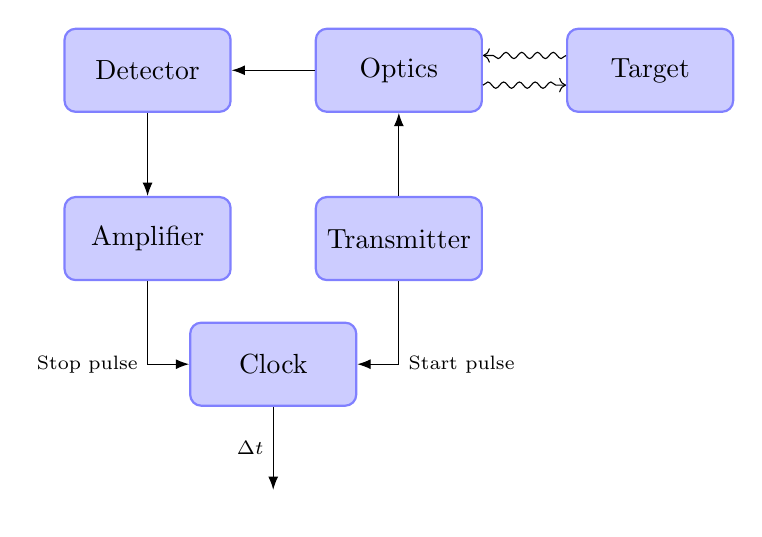
\begin{tikzpicture}[
    block/.style={rectangle,thick,
        draw=blue!50,
        fill=blue!20, 
        rounded corners, 
        text centered, 
        minimum height = 3em, 
        minimum width=6em},
        on grid=false,
        node distance=3em,
        auto,
    ]

    \node [block] (detector) {Detector};
    \node [block, below = of detector] (amplifier) {Amplifier};
    \node [block, right = of amplifier] (transmitter) {Transmitter};
    \node [block, below = of $(amplifier)!0.5!(transmitter)$] (timer)  {Clock};
    \node [block, right = of detector] (beamsplitter) {Optics};
    \node [block, right = of beamsplitter] (target) {Target};
    
    \node [below = of timer] (system) {};

    \draw[-Latex] (amplifier) |- node[left] {\scriptsize Stop pulse}  (timer.west);
    \draw[-Latex] (transmitter.south) |- node[right] {\scriptsize Start pulse} (timer.east);
    \draw[-Latex] (detector.south) -- (amplifier.north);

    \draw[-Latex] (transmitter.north) -- (beamsplitter.south);
    \draw[->,decorate,
        decoration={snake,amplitude=.4mm,segment length=2mm,post length=1mm}] (beamsplitter.350) -- (target.190);
    \draw[->,decorate,
        decoration={snake,amplitude=.4mm,segment length=2mm,post length=1mm}] (target.170) -- (beamsplitter.10);

    \draw[-Latex] (beamsplitter) -- (detector);
    \draw[-Latex] (timer) -- node[left] {\scriptsize $\Delta t$} (system);
\end{tikzpicture}
\end{document}
